\documentclass{article}

\usepackage{amsmath,amssymb}
\usepackage{tikz}
\usepackage{pgfplots}
\usepackage{xcolor}
\usepackage[left=2.1cm,right=3.1cm,bottom=3cm,footskip=0.75cm,headsep=0.5cm]{geometry}
\usepackage{enumerate}
\usepackage{enumitem}
\usepackage{marvosym}
\usepackage{tabularx}
\usepackage{multirow}

\usepackage{listings}
\definecolor{lightlightgray}{rgb}{0.95,0.95,0.95}
\definecolor{lila}{rgb}{0.8,0,0.8}
\definecolor{mygray}{rgb}{0.5,0.5,0.5}
\definecolor{mygreen}{rgb}{0,0.8,0.26}
\lstdefinestyle{java} {language=java}
\lstset{language=java,
	basicstyle=\ttfamily,
	keywordstyle=\color{lila},
	commentstyle=\color{lightgray},
	stringstyle=\color{mygreen}\ttfamily,
	backgroundcolor=\color{white},
	showstringspaces=false,
	numbers=left,
	numbersep=10pt,
	numberstyle=\color{mygray}\ttfamily,
	identifierstyle=\color{blue},
	xleftmargin=.1\textwidth, 
	%xrightmargin=.1\textwidth,
	escapechar=§,
}

\usepackage[utf8]{inputenc}

\renewcommand*{\arraystretch}{1.4}

\newcolumntype{L}[1]{>{\raggedright\arraybackslash}p{#1}}
\newcolumntype{R}[1]{>{\raggedleft\arraybackslash}p{#1}}
\newcolumntype{C}[1]{>{\centering\let\newline\\\arraybackslash\hspace{0pt}}m{#1}}

\newcommand{\E}{\mathbb{E}}
\DeclareMathOperator{\rk}{rk}
\DeclareMathOperator{\Var}{Var}
\DeclareMathOperator{\Cov}{Cov}

\title{\textbf{Grundlagen des Finanzmanagements, Tutorium 2}}
\author{\textsc{Henry Haustein}}
\date{}

\begin{document}
	\maketitle
	
	\section*{Aufgabe 6.2: Cashflows, Preise und Renditen von Anleihen}
	\begin{enumerate}[label=(\alph*)]
		\item Die Effektivverzinsungen sind
		\begin{itemize}
			\item 1-Jahres-Anleihe: $\frac{100}{95.51}-1 = 0.047$
			\item 2-Jahres-Anleihe: $\sqrt{\frac{100}{91.05}}-1 = 0.048$
			\item 3-Jahres-Anleihe: $\sqrt[3]{\frac{100}{86.38}}-1 = 0.050$
			\item 4-Jahres-Anleihe: $\sqrt[4]{\frac{100}{81.65}}-1 = 0.052$
			\item 5-Jahres-Anleihe: $\sqrt[5]{\frac{100}{76.51}}-1 = 0.055$
		\end{itemize}
		\item Graph
		\begin{center}
			\begin{tikzpicture}
				\begin{axis}[
					xmin=0, xmax=5, xlabel={Restlaufzeit},
					ymin=0, ymax=0.06, ylabel={Effektivverzinsung},
					samples=400,
					axis x line=middle,
					axis y line=middle,
					domain=0:5,
					]
					\addplot[mark=x,blue] coordinates {
						(1,0.047)
						(2,0.048)
						(3,0.050)
						(4,0.052)
						(5,0.055)
					};
					
				\end{axis}
			\end{tikzpicture}
		\end{center}
		\item steigend
	\end{enumerate}
	
	\section*{Aufgabe 6.5: Cashflows, Preise und Renditen von Anleihen}
	\begin{enumerate}[label=(\alph*)]
		\item Die Effektivverzinsung ist
		\begin{align}
			P &= \frac{K}{y}\left(1-\frac{1}{(1+y)^N}\right) + \frac{NOM}{(1+y)^N} \notag \\
			1034.74 &= \frac{80}{y}\left(1-\frac{1}{(1+y)^{10}}\right) + \frac{1000}{(1+y)^{10}} \notag \\
			y &= 0.0749 \notag
		\end{align}
		\item Der Preis ist
		\begin{align}
			P &= \frac{K}{y}\left(1-\frac{1}{(1+y)^N}\right) + \frac{NOM}{(1+y)^N} \notag \\
			&= \frac{80}{0.09}\left(1-\frac{1}{(1+0.09)^{10}}\right) + \frac{1000}{(1+0.09)^{10}} \notag \\
			&= 935.82 \notag
		\end{align}
	\end{enumerate}
	
	\section*{Aufgabe 6.9: Das Verhalten von Anleihepreisen}
	\begin{enumerate}[label=(\alph*)]
		\item Der Preis ist
		\begin{align}
			P &= \frac{K}{y}\left(1-\frac{1}{(1+y)^N}\right) + \frac{NOM}{(1+y)^N} \notag \\
			&= \frac{70}{0.06}\left(1-\frac{1}{(1+0.06)^{10}}\right) + \frac{1000}{(1+0.06)^{10}} \notag\\
			&= 1073.60 \notag
		\end{align}
		\item Unmittelbar vor der ersten Zahlung hat die Anleihe noch eine Restlaufzeit von 9 Jahren und es gibt eine Kuponzahlung. Also ist der Preis
		\begin{align}
			P &= 70 + \frac{K}{y}\left(1-\frac{1}{(1+y)^N}\right) + \frac{NOM}{(1+y)^N} \notag \\
			&= 70 + \frac{70}{0.06}\left(1-\frac{1}{(1+0.06)^{9}}\right) + \frac{1000}{(1+0.06)^{9}} \notag \\
			&= 1138.02 \notag
		\end{align}
		\item Nach der ersten Zahlung:
		\begin{align}
			P &= \frac{K}{y}\left(1-\frac{1}{(1+y)^N}\right) + \frac{NOM}{(1+y)^N} \notag \\
			&= \frac{70}{0.06}\left(1-\frac{1}{(1+0.06)^{9}}\right) + \frac{1000}{(1+0.06)^{9}} \notag \\
			&= 1068.02 \notag
		\end{align}
	\end{enumerate}

	\section*{Aufgabe 4K277: Fremdfinanzierung}
	\begin{enumerate}[label=(\alph*)]
		\item Wenn die Kreditsumme bei der DD-Bank 550.000 beträgt, dann muss nach einem Jahr maximal $550.000 + 55.000 = 605.000$ zurückgezahlt werden, was mit Sicherheit auch zurückgezahlt werden kann. Für die Investition sind dann noch 200.000 als Kredit von der EE-Bank aufzunehmen, dieser muss man nach einem Jahr $200.000 + 40.000 = 240.000$ zurückzahlen. Der erwartete Erlös sind
		\begin{align}
			\E(\text{Erlös}) &= 0.2\cdot 100.0000 + 0.3\cdot 900.000 + 0.3\cdot 750.000 + 0.2\cdot 605.000 \notag \\
			&= 816.´000 \notag
		\end{align}
		Von diesem erwarteten Erlös gehen 605.000 an die DD-Bank, es bleiben 211.000 für die EE-Bank. Das sind weniger als die benötigten 240.000, die EE-Bank wird also keine Finanzierung durchführen. In den einzelnen Zuständen erreicht die EE-Bank folgende Verzinsung:
		\begin{itemize}
			\item Misserfolg: Der Erlös geht zu 100\% an die DD-Bank, die EE-Bank verdient nichts, ihre 200.000 sind weg. Die Verzinsung beträgt somit $\frac{-200.000}{200.000} = -1$.
			\item schlechter Erfolg: Nach Bezahlung der Schulden bei der DD-Bank bleiben 145.000 für die EE-Bank, also ein Verlust von 55.000. Die Verzinsung ist $\frac{-55.000}{200.000}=-0.275$.
			\item mittlerer Erfolg: Für die EE-Bank bleiben 295.000, also ist die Verzinsung $\frac{95.000}{200.000}=0.475$.
		\end{itemize}
		Die erwartete Verzinsung soll 20\% betragen, also
		\begin{align}
			0.2 &= 0.2\cdot -1 + 0.3\cdot -0.275 + 0.3 \cdot 0.475 + 0.2\cdot x \notag \\
			x &= 1.7 \notag
		\end{align}
		Die EE-Bank müsste also im großen Erfolgsfall 170\% Zinsen verlangen.
		\item Graph
		\begin{center}
			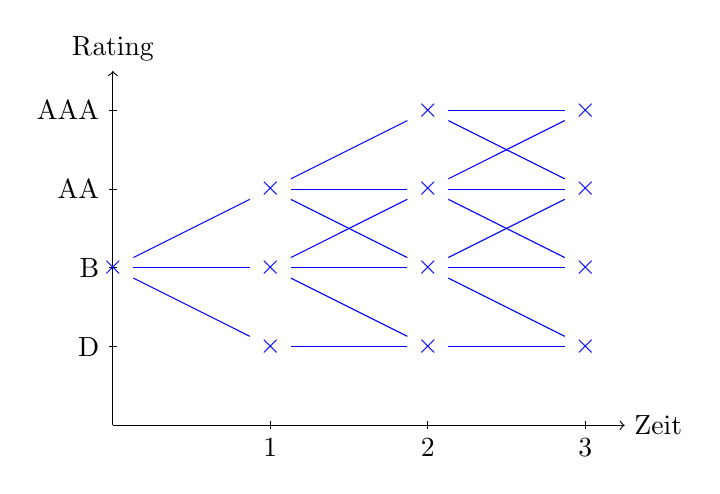
\begin{tikzpicture}
				\draw[->] (0,0) -- (6.5,0) node[right] {Zeit};
				\draw[->] (0,0) -- (0,4.5) node[above] {Rating};
				
				\draw (-0.05,1) node[left] {D} to (0.05,1);
				\draw (-0.05,2) node[left] {B} to (0.05,2);
				\draw (-0.05,3) node[left] {AA} to (0.05,3);
				\draw (-0.05,4) node[left] {AAA} to (0.05,4);
				
				\draw (2,0.05) -- (2,-0.05) node[below] {1};
				\draw (4,0.05) -- (4,-0.05) node[below] {2};
				\draw (6,0.05) -- (6,-0.05) node[below] {3};
				
				\node[blue] at (0,2) (a2) {$\times$};
				
				\node[blue] at (2,1) (b1) {$\times$};
				\node[blue] at (2,2) (b2) {$\times$};
				\node[blue] at (2,3) (b3) {$\times$};
				
				\node[blue] at (4,1) (c1) {$\times$};
				\node[blue] at (4,2) (c2) {$\times$};
				\node[blue] at (4,3) (c3) {$\times$};
				\node[blue] at (4,4) (c4) {$\times$};
				
				\node[blue] at (6,1) (d1) {$\times$};
				\node[blue] at (6,2) (d2) {$\times$};
				\node[blue] at (6,3) (d3) {$\times$};
				\node[blue] at (6,4) (d4) {$\times$};
				
				\draw[blue] (a2) -- (b1);
				\draw[blue] (a2) -- (b2);
				\draw[blue] (a2) -- (b3);
				
				\draw[blue] (b1) -- (c1);
				\draw[blue] (b2) -- (c1);
				\draw[blue] (b2) -- (c2);
				\draw[blue] (b2) -- (c3);
				\draw[blue] (b3) -- (c2);
				\draw[blue] (b3) -- (c3);
				\draw[blue] (b3) -- (c4);
				
				\draw[blue] (c1) -- (d1);
				\draw[blue] (c2) -- (d1);
				\draw[blue] (c2) -- (d2);
				\draw[blue] (c2) -- (d3);
				\draw[blue] (c3) -- (d2);
				\draw[blue] (c3) -- (d3);
				\draw[blue] (c3) -- (d4);
				\draw[blue] (c4) -- (d3);
				\draw[blue] (c4) -- (d4);
			\end{tikzpicture}
		\end{center}
		\item Die Wahrscheinlichkeit, dass die Anleihe immer bei B bleibt, ist $0.4^3=0.064$. Sei $A$ die Übergangsmatrix, also
		\begin{align}
			A = \begin{pmatrix}
				0.2 & 0.8 & 0 & 0 \\
				0.1 & 0.5 & 0.4 & 0 \\
				0 & 0.3 & 0.4 & 0.3 \\
				0 & 0 & 0 & 1
			\end{pmatrix} \notag
		\end{align}
		Die Wahrscheinlichkeiten für ein bestimmtes Rating nach 3 Perioden, wenn die Anleihe bei B gestartet ist, ist
		\begin{align}
			\begin{pmatrix}
				0 \\ 0 \\ 1 \\ 0
			\end{pmatrix} \cdot A^3 = \begin{pmatrix}
				0.033 \\ 0.243 \\ 0.22 \\ 0.504
			\end{pmatrix} \notag
		\end{align}
		Die Wahrscheinlichkeit für ein AAA-Rating ist also 0.033.
		\item Nach 2 Perioden ist die Wahrscheinlichkeitsverteilung
		\begin{align}
			\begin{pmatrix}
				0 \\ 0 \\ 1 \\ 0
			\end{pmatrix} \cdot A^2 = \begin{pmatrix}
				0.03 \\ 0.27 \\ 0.28 \\ 0.42
			\end{pmatrix} \notag
		\end{align}
		\item Nach einem Jahr hat die Anleihe mit einer Wahrscheinlichkeit von 0.3 ein D-Rating. Nach 3 Jahren ist sie es mit einer Wahrscheinlichkeit von 0.504 (siehe (c)).
		\item Die erwartete Auszahlung in den einzelnen Jahren ist
		\begin{itemize}
			\item 1. Jahr: $(0.3 + 0.4)\cdot 100 = 70$
			\item 2. Jahr: $(0.03 + 0.27 + 0.28)\cdot 100 = 58$
			\item 3. Jahr: $(0.033 + 0.243 + 0.22)\cdot 1100 = 545.6$
		\end{itemize}
		Der Preis für die Anleihe ist dann
		\begin{align}
			P &= \frac{70}{1.05} + \frac{58}{1.05^2} + \frac{545.6}{1.05^3} \notag \\
			&= 590.58 \notag
		\end{align}
	\end{enumerate}
	
	
\end{document}